\chapter{Resultados}\label{cap:results}

Este capítulo apresenta os resultados obtidos a partir da simulação da 
execução de trajetórias cartesianas para o manipulador 5R utilizando o esquema 
de controle RRC. Em cada cenário, foi realizado um conjunto de 4 execuções de 
uma mesma trajetória variando-se o ganho \(k_0\), com o objetivo de avaliar 
a eficácia do controlador em otimizar os índices de desempenho fornecidos, submetido 
a diferentes restrições cinemáticas.

\section{Cenário 1}

No primeiro cenário, a configuração do manipulador muda para trazer algumas posições 
das juntas o mais próximo possível de zero, enquanto a restrição primária imposta pela velocidade 
do efetuador final \(\xi = 0\) mantém a configuração final do manipulador numa solução particular, 
como podemos ver na figura \ref*{fig:exp1-joint-states}. A medida que aumentamos o ganho \(k_0\), a 
configuração do manipulador converge mais rapidamente para a solução final e na figura \ref*{fig:exp1-metric} 
podemos ver os valores menores da distância para os limites mecânicos das juntas sendo obtidos, ao custo 
de um valor de erro ligeiramente maior, como indicado na tabela \ref*{tab:scores-exp1}. Por fim, a figura 
\ref*{fig:exp1-position} mostra a posição do efetuador final constante ao longo de todo o experimento, 
mostrando que a restrição primária não é violada.

\begin{figure}
	\centering
	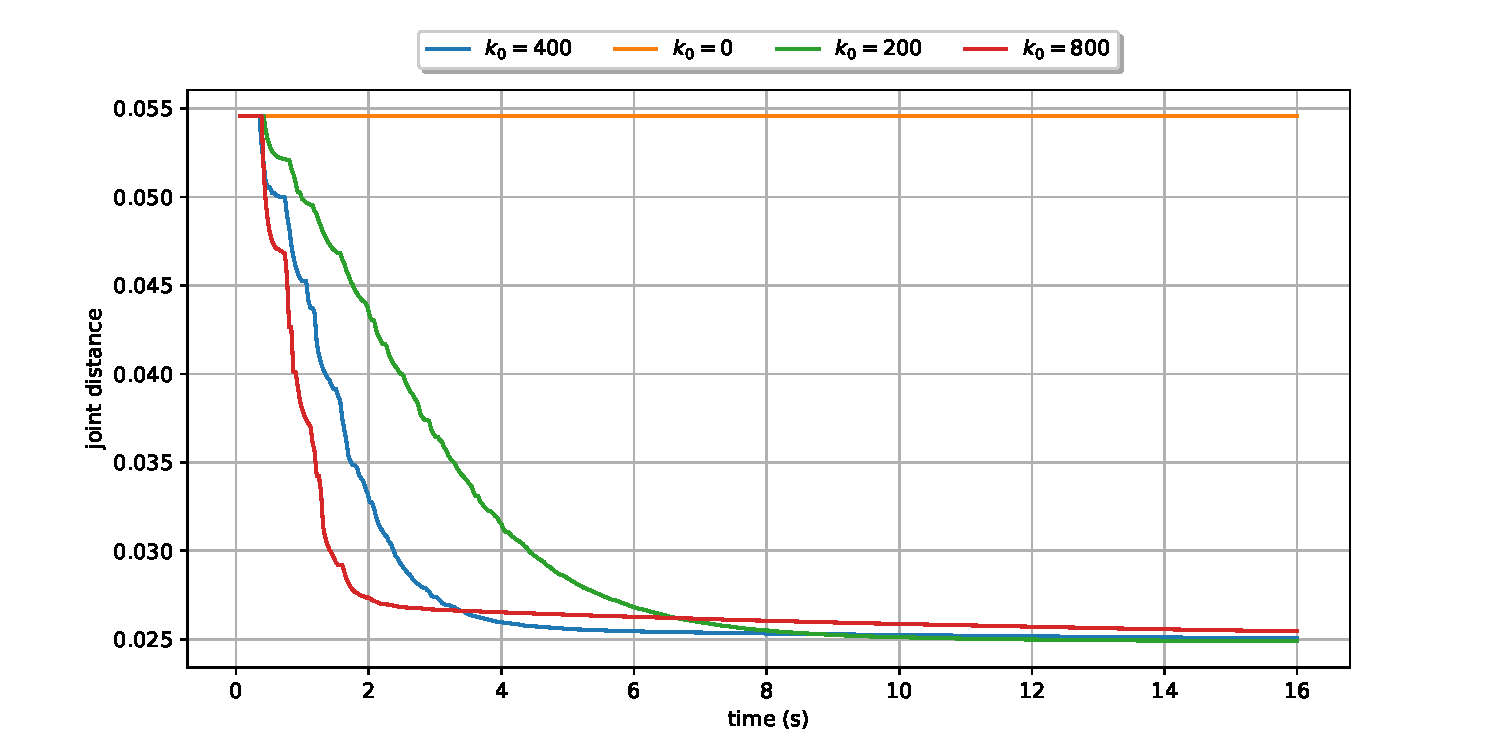
\includegraphics[width=\textwidth]{./Images/2024-06-11-09-23-42/metric_joint_distance.pdf}
	\caption{Diminuição da distância para o limite mecânico das juntas ao longo tempo.}\label{fig:exp1-metric}
\end{figure}

\begin{figure}
	\centering
	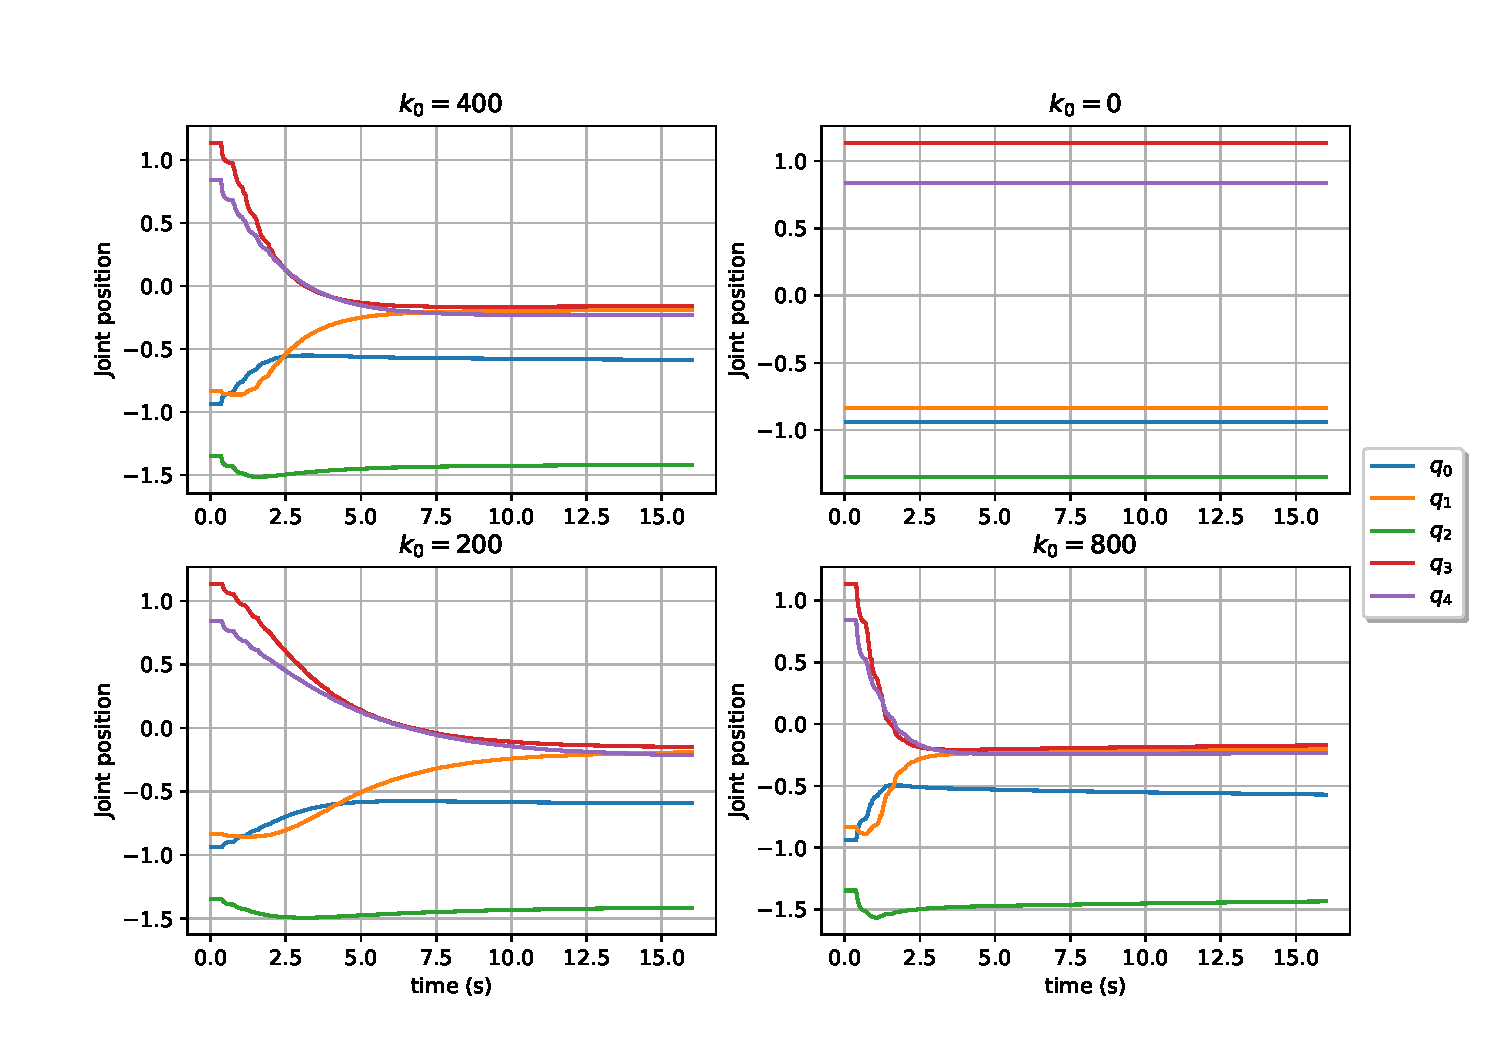
\includegraphics[width=\textwidth]{./Images/2024-06-11-09-23-42/joint_states_joint_distance.pdf}
	\caption{Diferentes valores do ganho, influenciam diretamente na velocidade de convergência para a solução particular.}\label{fig:exp1-joint-states}
\end{figure}

\begin{figure}
	\centering
	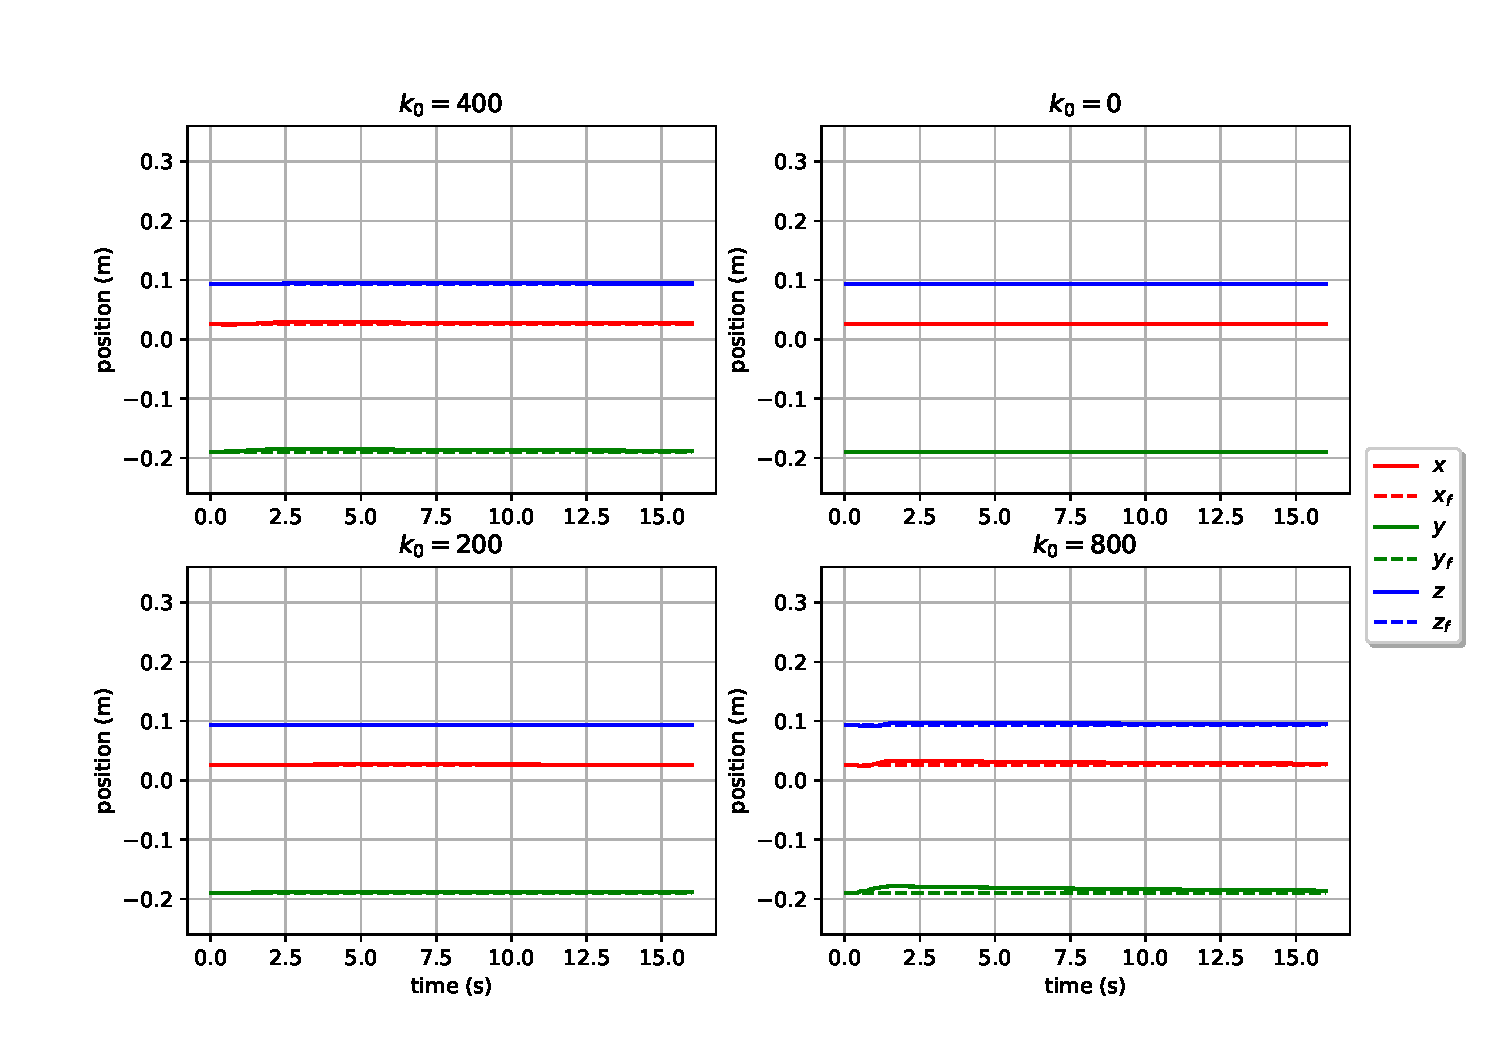
\includegraphics[width=\textwidth]{./Images/2024-06-11-09-23-42/position_joint_distance.pdf}
	\caption{Posição do efetuador final mantém-se constante ao longo do tempo, devido à restrição primária.}\label{fig:exp1-position}
\end{figure}

\begin{table}[htbp]
    \centering
    \begin{tabular}{ccc}
        \toprule
        \( k_0 \) & \( I(w) \)  & Erro posição (m) \\
        \midrule
        0  & \( 0.8729 \) & \( \textbf{1.8535e-06} \) \\
        200  & \( 0.4829 \) & \( 0.0013 \) \\
        400  & \( 0.4488 \) & \( 0.0023 \) \\
        800  & \( \textbf{0.4435} \) & \( 0.0048 \) \\
        \bottomrule
    \end{tabular}
    \caption{Valores de desempenho obtidos na execução dos experimentos do primeiro cenário.}
    \label{tab:scores-exp1}
\end{table}

\section{Cenário 2}
	
No segundo cenário, com a introdução de uma velocidade inicial não nula do efetuador final, isto é \(||\xi|| > 0 \), 
a manipulabilidade muda ao longo da execução da trajetória, aproximando-se de um valor mínimo no seu final (figura \ref*{fig:exp2-metric}). 
A resolução de redundância atualiza a configuração do manipulador de modo manter a manipulabilidade o mais 
alta possível, sem violar a restrição primária.

Observamos novamente que o efeito de introduzir valores crescentes do ganho afeta o erro de posição 
com um pequeno \emph{trade-off} entre a otimização da métrica e a precisão no controle da posição 
do efetuador final (tabelas \ref*{tab:scores-exp2} e \ref*{tab:scores-exp3}), tendo em vista o aumento das 
velocidades das juntas. Esse fenômeno pode ser melhor observado nas figuras \ref*{fig:exp3-joint-states} e 
\ref*{fig:exp3-error}, onde a velocidade das juntas aumenta significativamente ao longo da execução da trajetória, 
e o erro se mantém maior a medida que o ganho \(k_0\) aumenta. Isso pode ser explicado pelo fato 
de que a métrica de desempenho, nesse caso a distância das juntas (figura \ref*{fig:exp3-metric}), é otimizada como um objetivo secundário 
à restrição imposta por \(\xi\), e a escolha de trajetórias onde os valores da métricas estão muito distantes
 do valor ótimo, acabam tornando o processo de otimização mais difícil, necessitando assim um valor de \(k_0\) 
 maior para convergir para a solução ótima.

\begin{figure}
	\centering
	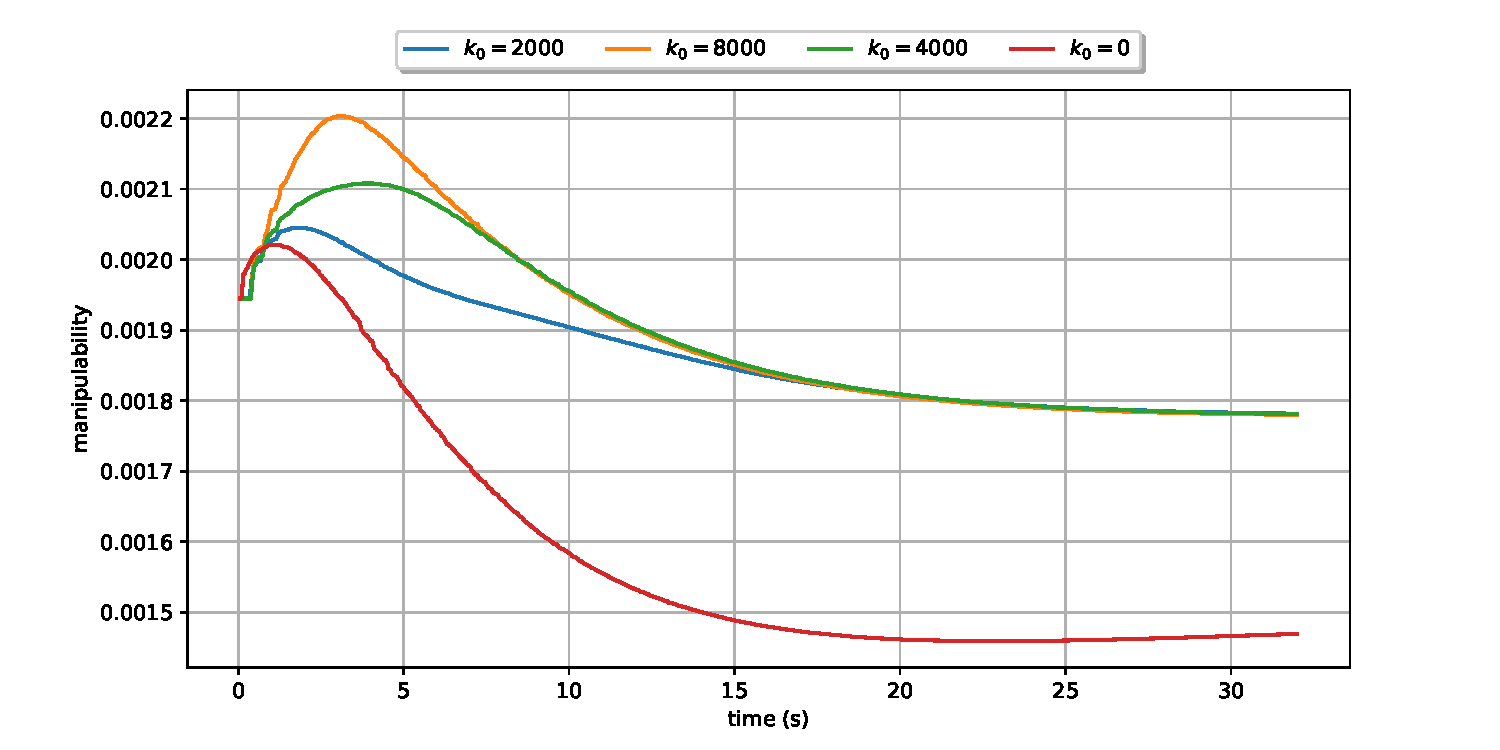
\includegraphics[width=\textwidth]{./Images/2024-06-11-09-17-48/metric_manipulability.pdf}
	\caption{Manipulabilidade em função do tempo para cada trajetória executada no segundo cenário.}\label{fig:exp2-metric}
\end{figure}

\begin{table}[htbp]
    \centering
    \begin{tabular}{ccc}
        \toprule
        \( k_0 \) & \( I(w) \)  & Erro posição (m) \\
        \midrule
        0  & \( 0.0507 \) & \( \textbf{0.0138} \) \\
        2000  & \( 0.0597 \) & \( 0.0150 \) \\
        4000  & \( 0.0606 \) & \( 0.0151 \) \\
        8000  & \( \textbf{0.0609} \) & \( 0.0149 \) \\
        \bottomrule
    \end{tabular}
    \caption{Valores de desempenho obtidos na execução dos experimentos do segundo cenário.}
    \label{tab:scores-exp2}
\end{table}

\begin{figure}
	\centering
	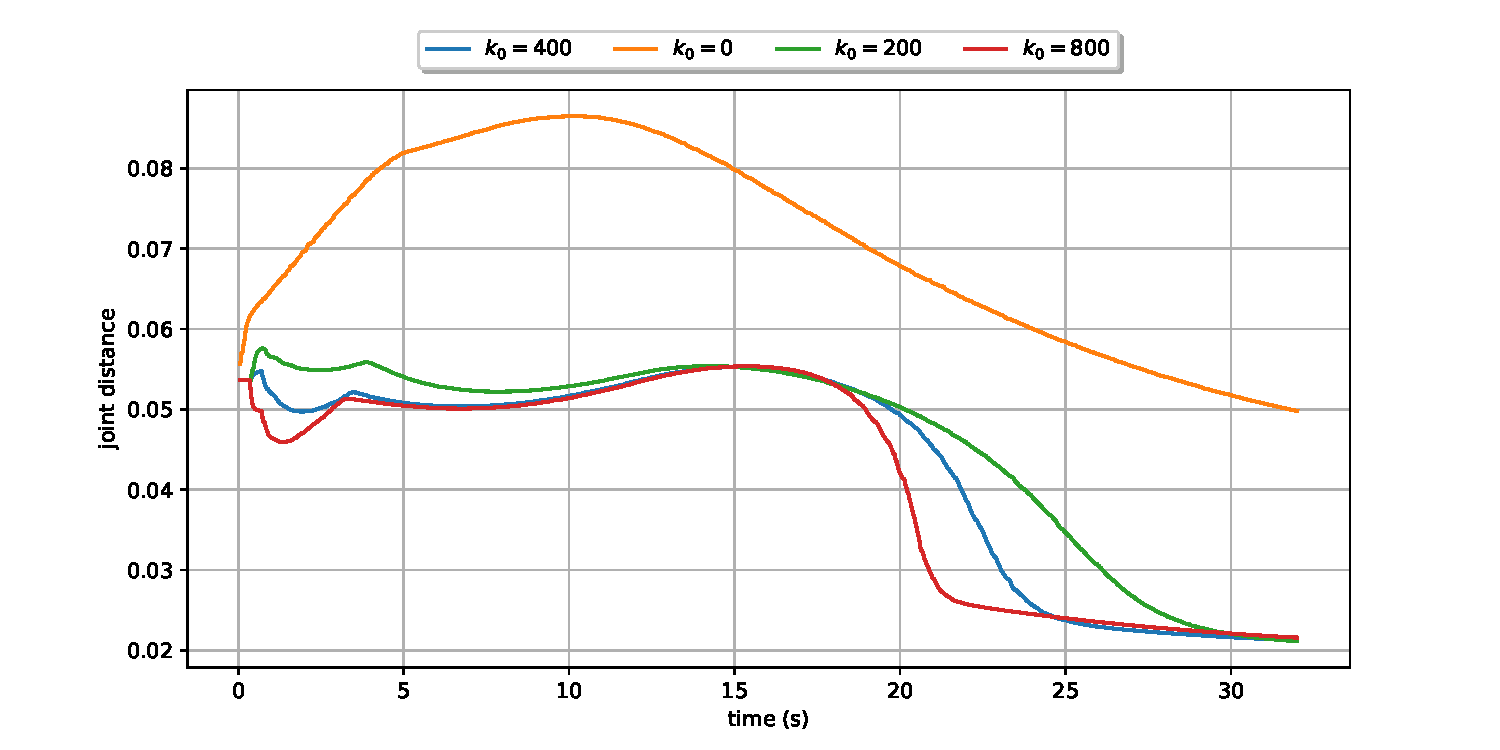
\includegraphics[width=\textwidth]{./Images/2024-07-02-14-04-38/metric_joint_distance.pdf}
	\caption{Otimizando distância das juntas no segundo cenário.}\label{fig:exp3-metric}
\end{figure}

\begin{figure}
	\centering
	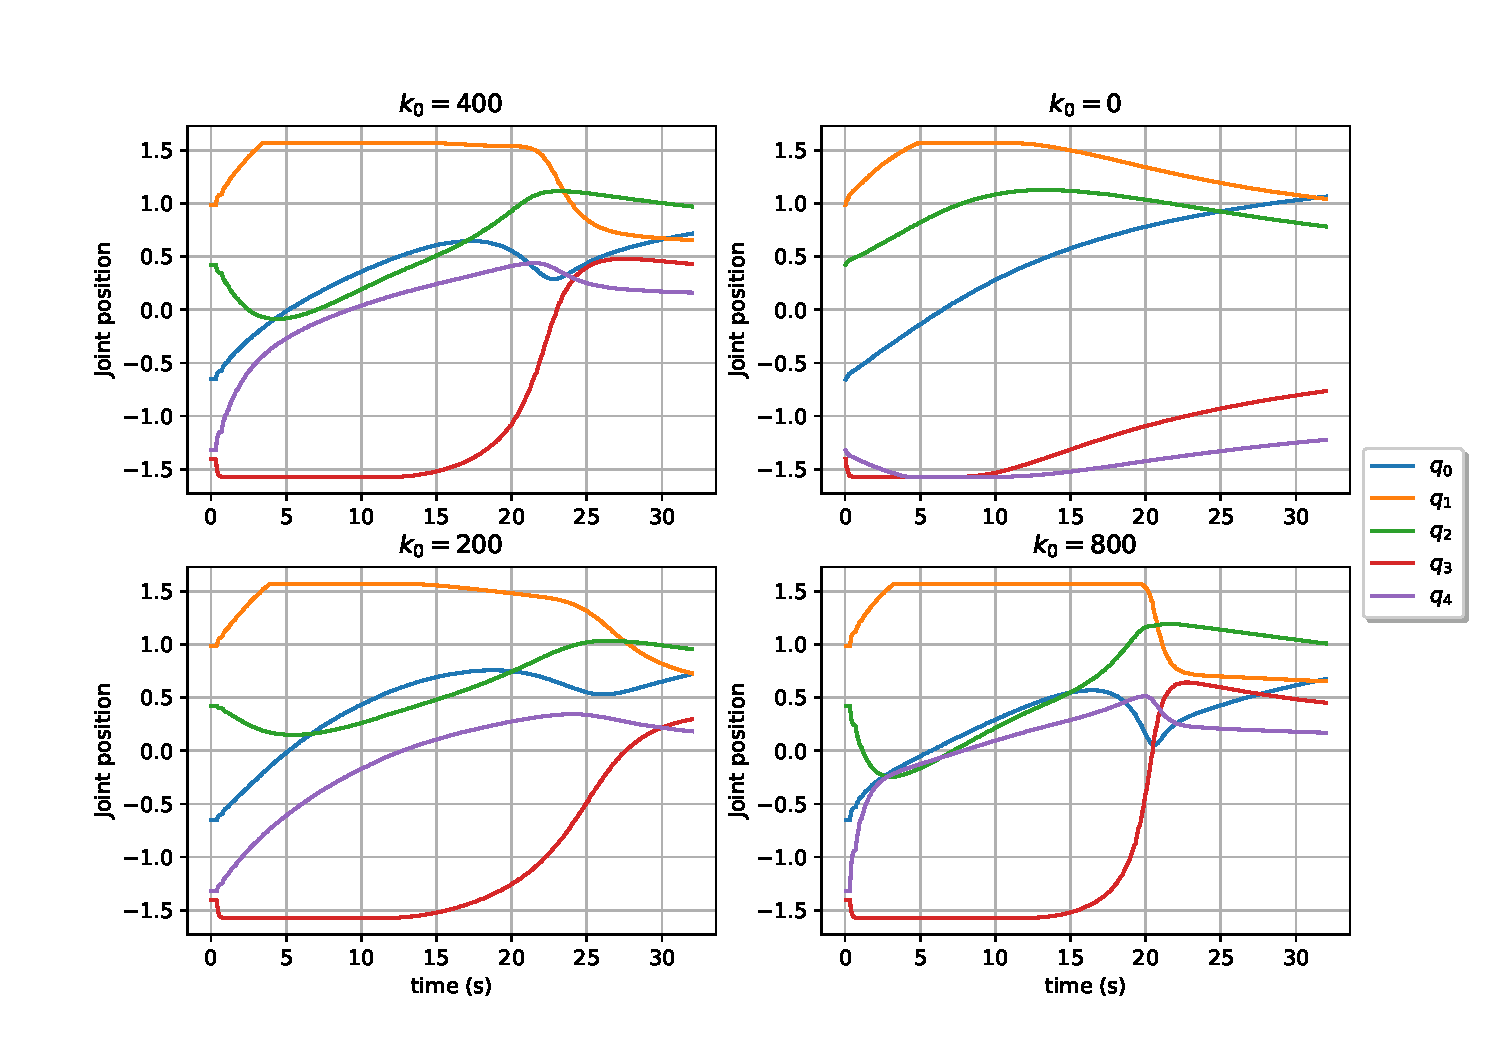
\includegraphics[width=\textwidth]{./Images/2024-07-02-14-04-38/joint_states_joint_distance.pdf}
	\caption{Em determinadas trajetórias, o impacto do ganho na velocidade das juntas é significativo.}\label{fig:exp3-joint-states}
\end{figure}

\begin{figure}
	\centering
	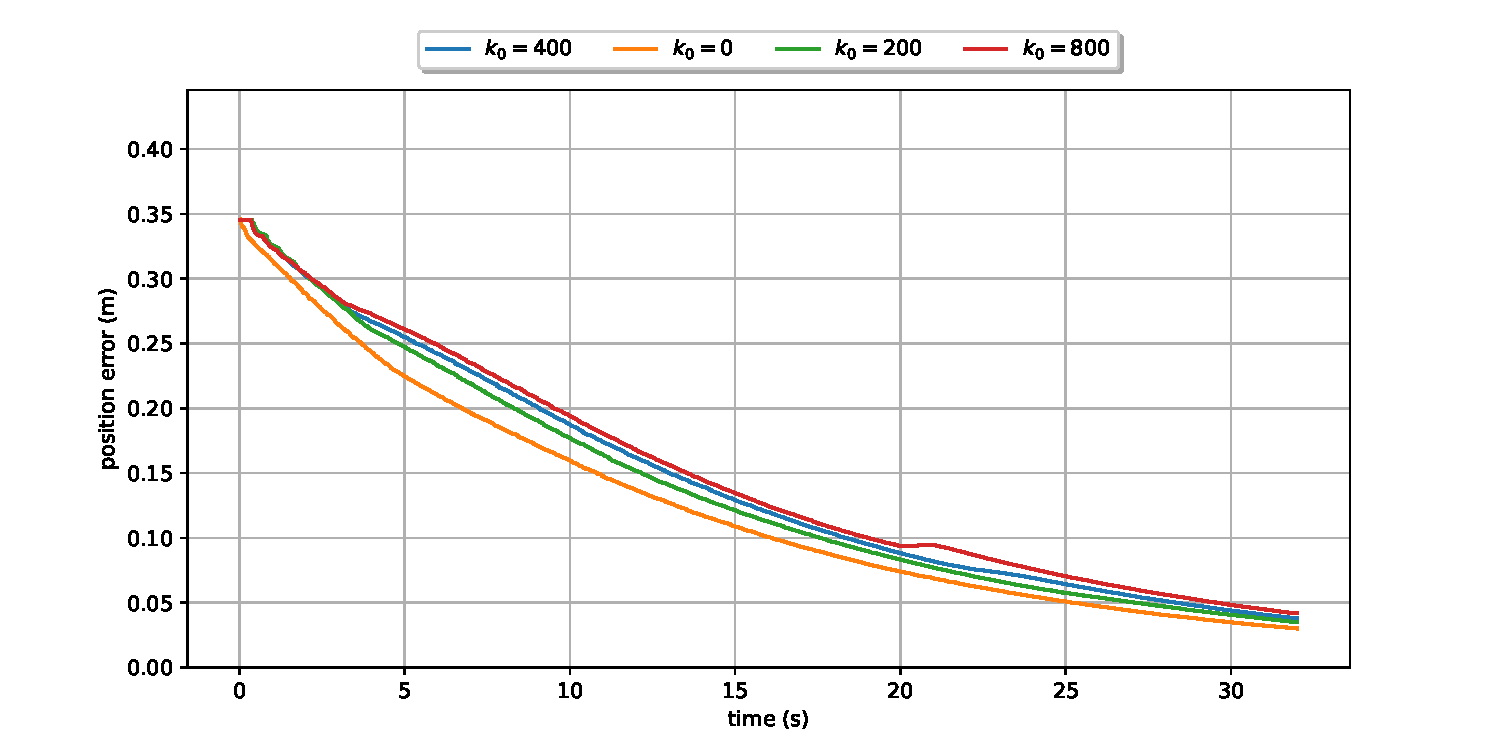
\includegraphics[width=\textwidth]{./Images/2024-07-02-14-04-38/position_error_joint_distance.pdf}
	\caption{Erro da posição ao longo do tempo para o segundo cenário.}\label{fig:exp3-error}
\end{figure}

\begin{table}[htbp]
    \centering
    \begin{tabular}{ccc}
        \toprule
        \( k_0 \) & \( I(w) \) & Erro posição (m) \\
        \midrule
        0  & \( 2.2622 \) & \( \textbf{0.0301} \) \\
        200  & \( 1.4727 \) & \( 0.0350 \) \\
        400  & \( 1.3777 \) & \( 0.0379 \) \\
        800  & \( \textbf{1.3251} \) & \( 0.0418 \) \\
        \bottomrule
    \end{tabular}
    \caption{Valores de desempenho (métrica distância das juntas) obtidos na execução dos experimentos no segundo cenário.}
    \label{tab:scores-exp3}
\end{table}
